\documentclass[10pt]{article}

\usepackage[top=0.5in, bottom=0.5in, left=0.5in, right=0.5in]{geometry}
\usepackage{authblk}
\usepackage{hyperref}
\usepackage[utf8]{inputenc}
\usepackage{amsmath}
\usepackage{amsfonts}
\usepackage{amssymb}
\usepackage{siunitx}
\usepackage{graphicx}
\usepackage{subcaption}
\usepackage{float}
\usepackage[nottoc,numbib]{tocbibind}
\usepackage{biblatex}
\usepackage{graphicx,wrapfig,lipsum} % For Figures

% For Diagrams
\usepackage{tikz}

\bibliography{references.bib}

\newcommand{\email}[1]{\texttt{\href{mailto:#1}{#1}}}

\title{A Deep Learning Approach to Finding the Initial Conditions of the Universe}

\makeatletter
\let\inserttitle\@title
\makeatother

\begin{document}

\begin{center}
  \LARGE{\inserttitle}
\end{center}

\noindent
PI: Aarti Singh\footnote{Associate Professor, Machine Learning Department, Carnegie Mellon University, \email{aarti@cs.cmu.edu}}. CoPI: Shirley Ho\footnote{Group Leader, Center for Computational Astrophysics, Flatiron Institute, \email{shirleyho@flatironinstitute.org}}

\noindent
User: Albert Liang\footnote{Graduate student, Machine Learning Department, Carnegie Mellon University, \email{ajliang@cs.cmu.edu}}, Vaibhav Jindal\footnote{Graduate Student, Machine Learning Department, Carnegie Mellon University, \email{vjindal@cs.cmu.edu}}}

\section{Abstract}

This work introduces a novel neural-network based model to predict the linear inputs of an N-body simulation given its non-linear displacement at redshift zero.
Specifically, our method is based on a convolutional neural network with a V-Net-like architecture, which is trained to output the linear displacement of an N-body system, given the current time non-linear displacement and the corresponding cosmological parameters.
We call this model the \textit{Inverse Modeling} network, or simply the backward model.
Since the mapping between the non-linear displacements to the linear displacements is one-to-many, training a neural network for such predictions is essentially ill-defined because of the one-to-one nature of neural network mappings.
However, in this work, we demonstrate that neural networks can accurately recover the initial displacement field on large scales despite the ill-defined nature of the problem.
This is the first work that tries to use a neural network to predict the initial conditions of the universe given the current time conditions.
Due to limited computational resources, at the moment, we have only tested our method on a small set of synthetic N-body simulations. However, these preliminary results have already shown great promises and we are looking to utilize more powerful GPUs to further train and evaluate our backward model on larger, more realistic simulations such as the Quijote simulation suite \cite{quijote}. Specifically, we hope to get approved for Accelerate ACCESS credits so that we can access $\geq 4$ GPUs with $\geq 32$ GB of memory on a cluster with $7$TB of disk space. We plan to use our credits at PSC (Pittsburgh Supercomputing Center).

\section{Introduction}

The evolution of our universe can be uniquely determined by its initial conditions and the laws of physics governing its dynamics. To understand the evolution of  universe, astrophysicists use a large number of simulations to extract meaningful information. These simulations try to predict the non-linear structure of a system of N-body particles given the initial conditions of these particles. These forward simulations, however, are computationally expensive and require a large amount of time.

In recent years, deep-learning has shown to be extremely helpful in accelerating the forward modeling process \cite{he_li_feng_ho_ravanbakhsh_chen_póczos_2019}. These deep-learning models learn from pairs of inputs and outputs from actual physical N-body simulations and act as fast and accurate approximators for these simulators. These deep learning surrogates speed up the forward modelling process by orders of magnitude. Since neural networks are theoretically proven to be universal function approximators, the forward modeling of N-body simulations fits perfectly into the regime of neural networks.

\begin{wrapfigure}{r}{0.4\textwidth}
  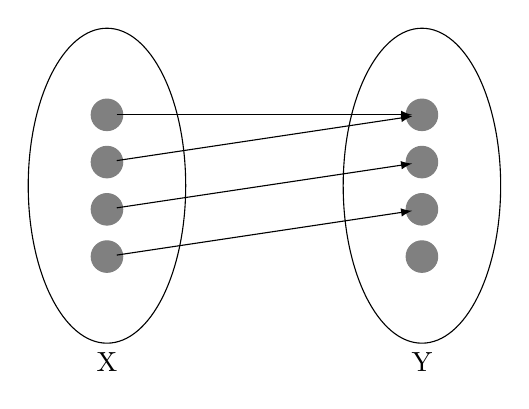
\begin{tikzpicture}
    % Set X oval
    \draw (-2,0) ellipse (1 and 2);
    \draw (-2,-2) node[below] {X};
    % Set X elements
    \draw[gray, fill=gray] (-2,0.9) circle (0.2) node (x1) {};
    \draw[gray, fill=gray] (-2,0.3) circle (0.2) node (x2) {};
    \draw[gray, fill=gray] (-2,-0.3) circle (0.2) node (x3) {};
    \draw[gray, fill=gray] (-2,-0.9) circle (0.2) node (x4) {};

    % Set Y oval
    \draw (2,0) ellipse (1 and 2);
    \draw (2,-2) node[below] {Y};
    % Set Y elements
    \draw[gray, fill=gray] (2,0.9) circle (0.2) node (y1) {};
    \draw[gray, fill=gray] (2,0.3) circle (0.2) node (y2) {};
    \draw[gray, fill=gray] (2,-0.3) circle (0.2) node (y3) {};
    \draw[gray, fill=gray] (2,-0.9) circle (0.2) node (y4) {};

    % Arrows
    \draw[-latex] (x1) -- (y1);
    \draw[-latex] (x2) -- (y1);
    \draw[-latex] (x3) -- (y2);
    \draw[-latex] (x4) -- (y3);
  \end{tikzpicture}
    \caption{Example of a many-to-one function between two sets X and Y. For our purpose, X corresponds to the set of all possible initial conditions of an N-body simulation and Y corresponds to the set of final conditions.}
    \label{manytoone}
\end{wrapfigure}

The problem of inferring the initial state of the universe, or an N-body simulation, however poses a completely different challenge because multiple different initial states could lead to the same final state, i.e., it is a many-to-one function as demonstrated in Figure \ref{manytoone}. Thus, the mapping from final states to the initial states is not a function, but rather a one-to-many relation. Therefore, there is no direct way of determining the initial conditions and we must resort to sampling based optimization methods to infer possible initial states. Although counter-intuitive to the nature of the problem, we try to attack this problem by learning a deterministic neural network to output the initial states for a given output state. We show that despite the one-to-many nature of the mapping, a simple neural network, when trained to predict the initial state for a given output state, can do an excellent job of predicting the initial states at large scales. Our results empirically motivate the use of neural networks as approximate inverse-mapping black boxes that could generate reliable initial states for a given output state, which could then be used to speed up the more fine-grained sampling-based inverse modeling methods.

\section{Methods}

We train a V-Net based neural network to predict the initial state of an N-body system of particles evolving under gravity on an expanding cosmological background, given the final state. Our CNN takes the nonlinear displacement field at redshift $z=0$ and the value of the matter fraction $\mathbf{\Omega}_m$ as the input, and predicts the linear displacement field, i.e., the Zel'dovich approximation (ZA) at redshift $z=0$.

More formally, consider an N-body system with particles distributed on a uniform grid with positions $\mathbf{q}$. Let $\mathbf{\Psi}_{ZA}(\mathbf{q})$ be their linear ZA approximation at redshift $z=0$. Then, the final positions of the particles when they evolve linearly according to the Zel'dovich approximation is
$$\mathbf{x}_{lin}(\mathbf{q}) = \mathbf{q} + \mathbf{\Psi}_{ZA}(\mathbf{q}).$$
Let the final non-linear displacement of the particle initially at grid site $\mathbf{q}$ be $\mathbf{\Psi}_{NL}(\mathbf{q})$. Then, the final positions of the particles at redshift $z=0$ under non-linear evolution is
$$\mathbf{x}_{non-lin}(\mathbf{q}) = \mathbf{q} + \mathbf{\Psi}_{NL}(\mathbf{q}).$$
We train our V-Net model to output the linear displacement field $\mathbf{\Psi}_{ZA}(\mathbf{q})$ for a given non-linear displacement field $\mathbf{\Psi}_{NL}(\mathbf{q})$. Our V-Net model additionally takes the value of the matter fraction $\mathbf{\Omega}_m$ as an input, which can be thought of as a \textit{style} parameter. Similar to StyleGAN2 \cite{stylegan2}, the value of $\mathbf{\Omega}_m$ is multiplied with the convolutional kernels of each layer of the V-Net model. Note that this architecture is exactly equivalent to the \textit{style neural network} (SNN) architecture used in \cite{forward-model}.

Our training data consists of pairs of non-linear and linear displacement fields, which are synthetically generated from the style neural network that has already been fully trained in \cite{forward-model}. These displacement fields represent $128^3$ particles in a square box with a side-length of $250 h^{-1}$Mpc. The particles are distributed uniformly across this grid with a mean separation of $\sim1.95 h^{-1}$Mpc between two adjacent particles of the grid.

Our training procedures and hyperparameters are almost the same as the ones used in \cite{forward-model}, except that we reversed the inputs and outputs of the neural network. We now input the non-linear displacement field to our CNN and ask it to predict the linear displacement field. This is exactly opposite to what was being done by \cite{forward-model}.

\section{Preliminary Results on Synthetic Data}

\subsection{Qualitative Analysis}

\begin{wrapfigure}{r}{0.4\textwidth}
  \vspace{-1in}
  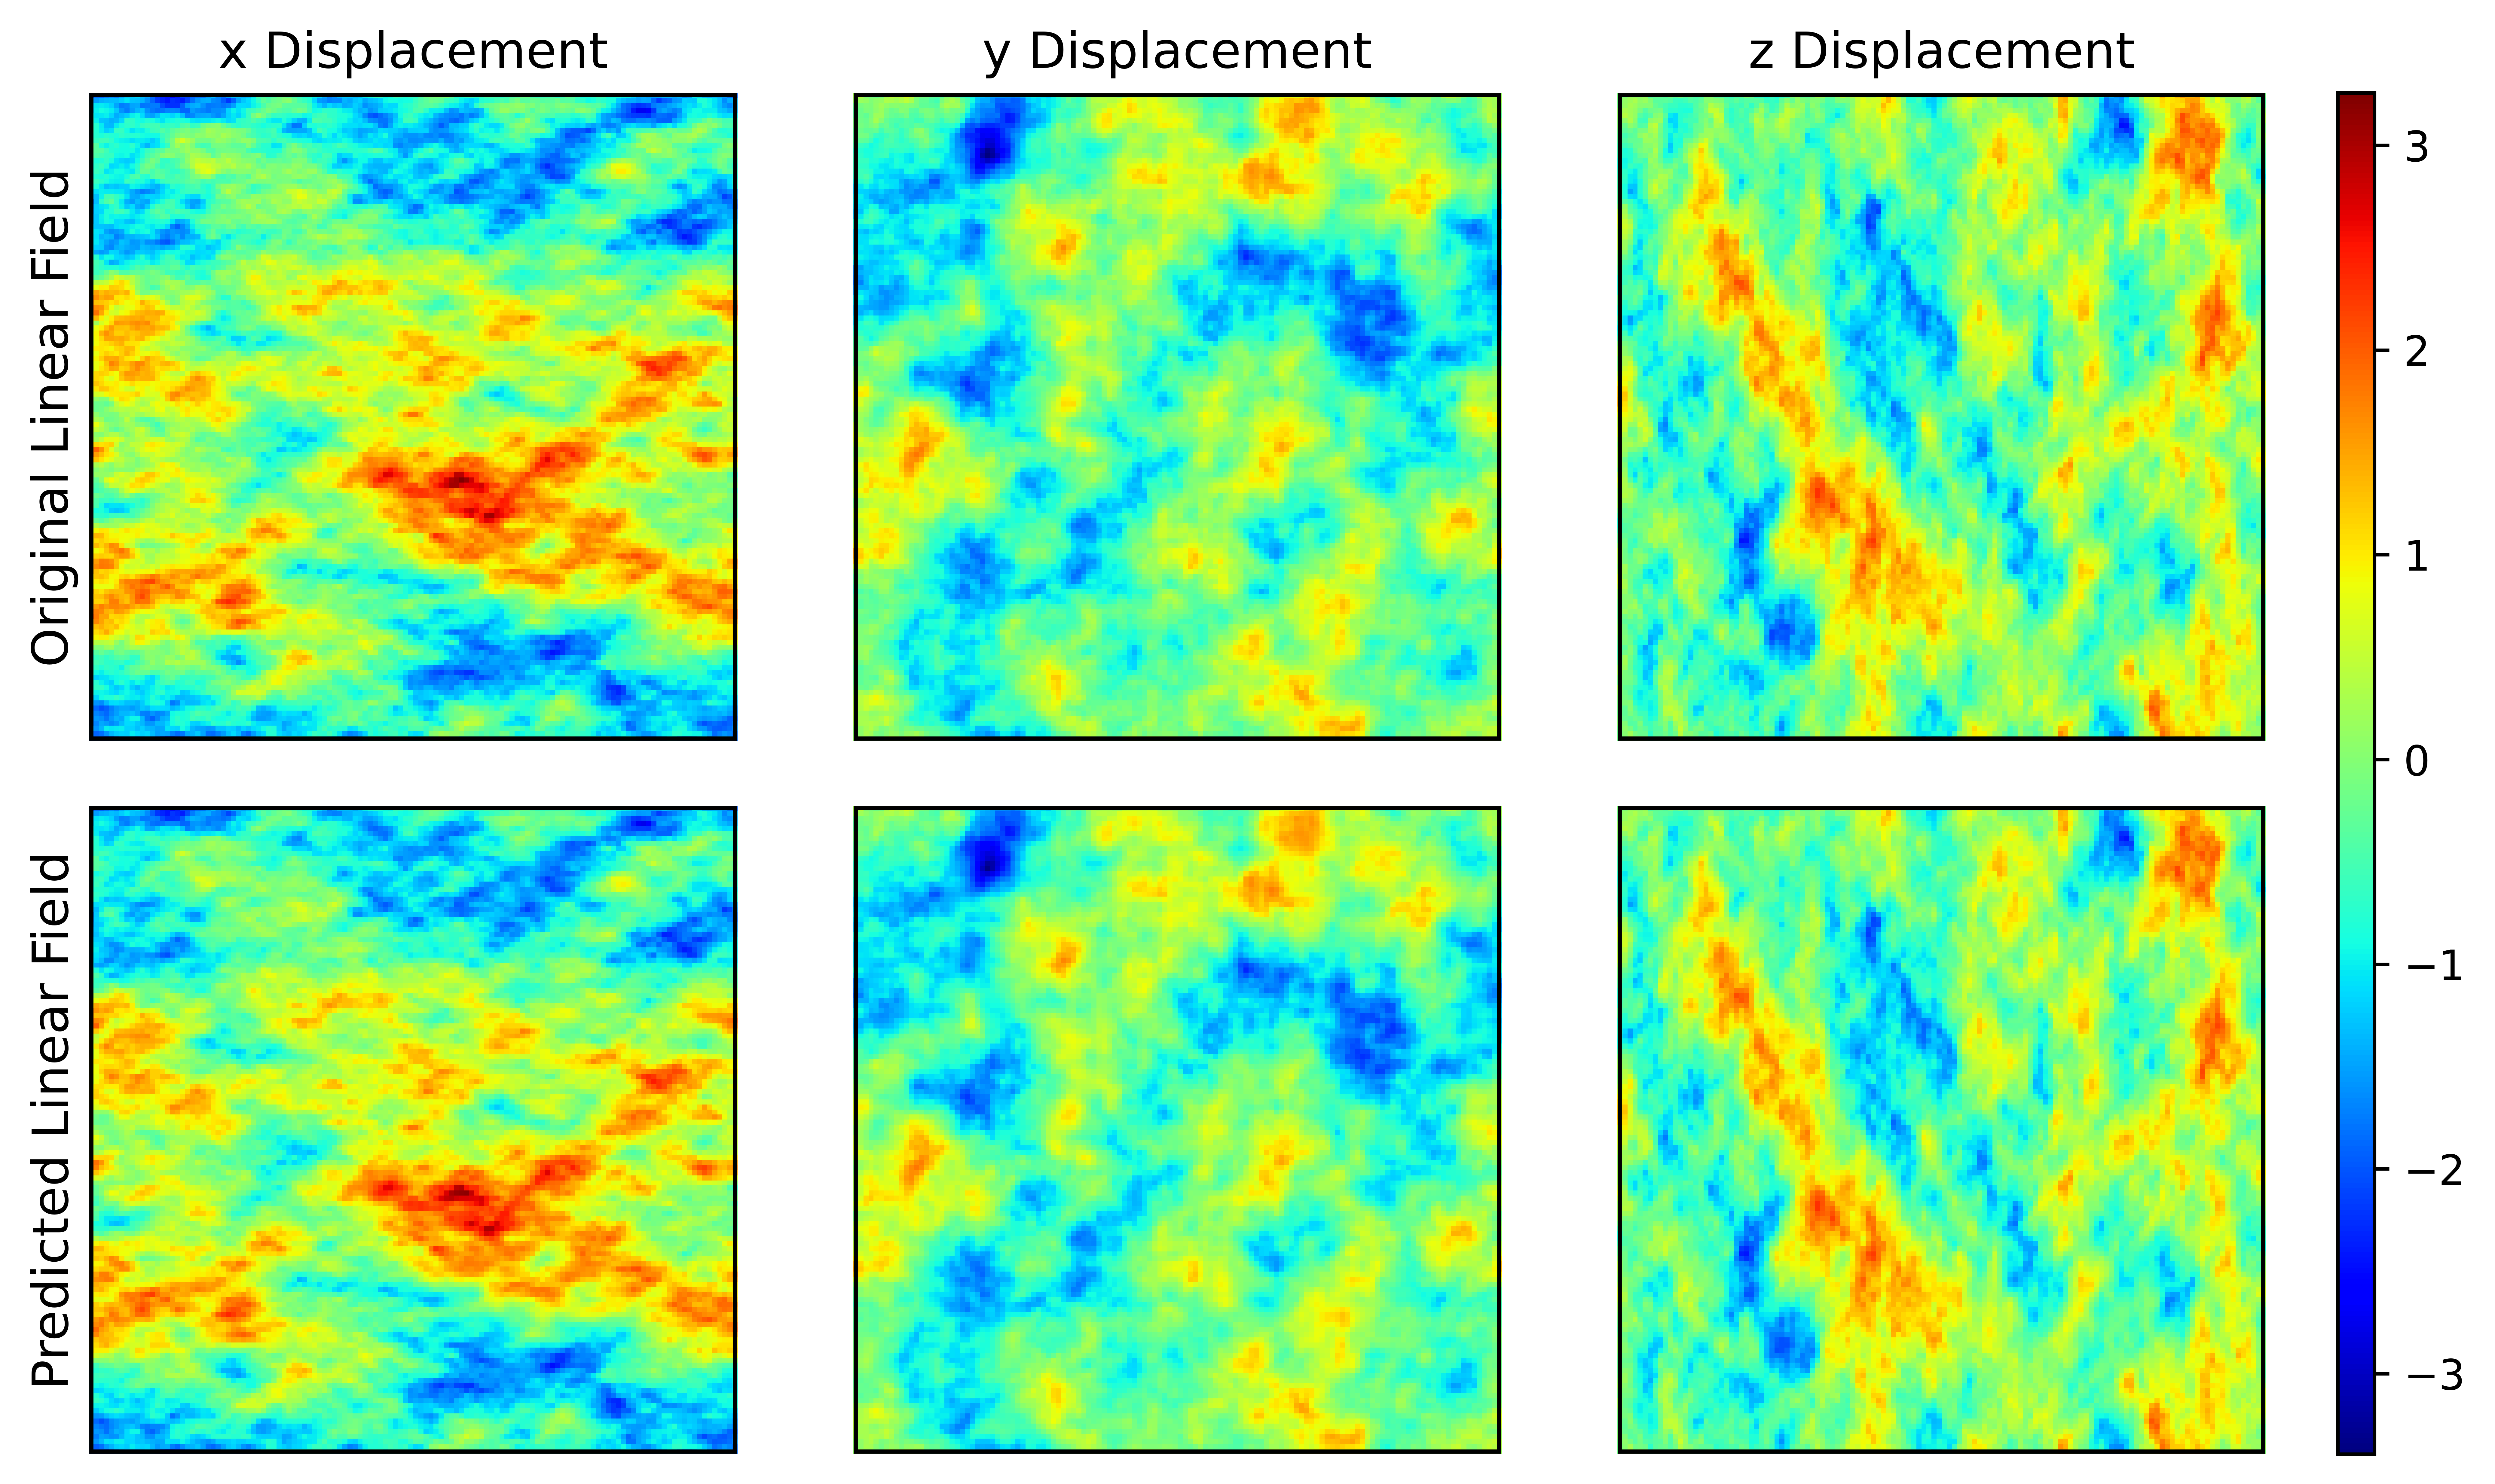
\includegraphics[width=0.4\textwidth]{images/slices.png}
  \caption{Qualitative comparison between a $128 \times 128$ slice of particles from the original linear field (target) and the corresponding linear field predicted by our inverse model (prediction). The plots show the $x,y, \text{and } z$ displacements for the two fields.}
  \label{slices}
\end{wrapfigure}


Figure \ref{slices} shows the x, y, and z direction displacements for a $128\times128$ slice of the original linear displacement field and the corresponding linear field predicted by our Inverse model. Qualitatively, the predictions of our model match very well with the original linear field that we wanted to predict.

\subsection{Two-Point Correlation Function}

\begin{figure*}[t!]
  \begin{center}
  \centerline{\includegraphics[width=\textwidth]{images/lin.png}}
  \caption{Two-point correlation comparison between the original linear displacement field (target) and the linear displacement field predicted by our model (prediction). For an exact prediction, the variation of power with wave number should be exactly the same for both the fields, and the values of transfer function fractional error and stochasticity should be exactly zero. }
  \label{lin}
  \end{center}
\end{figure*}

% \begin{figure*}[t!]
%   \begin{center}
%   \centerline{\includegraphics[width=\textwidth]{images/dis.png}}
%   \caption{Two-point correlation comparison between the original non-linear field (target) and the non-linear field generated from the predicted linear field given by the inverse model. For an exact prediction, the variation of power with wavenumber should be exactly similar for both the fields, and the values of transfer function fractional error and stochasticity should be exactly zero.}
%   \label{dis}
%   \end{center}
% \end{figure*}

The displacement power spectrum for a displacement field $\mathbf{\Psi}$ for wavenumber $k$ is defined as
$$
P(k) = \sum_{i \in \{x,y,z\}}\langle\mathbf{\Psi}_i(k)\mathbf{\Psi}_i(k)\rangle.
$$
Using this definition of power spectrum in the fourier space, we can now define the transfer function as
$$
T(k) = \sqrt{\frac{P_{pred}(k)}{P_{true}(k)}},
$$
and the correlation coefficient as
$$
r(k) = \frac{P_{pred \times true}(k)}{\sqrt{P_{pred}(k)P_{true}(k)}},
$$
where $P_{pred}(k)$ is the displacement power spectrum predicted by our neural network, $P_{true}(k)$ is the ground truth power spectrum and $P_{pred \times true}(k)$ is the cross power spectrum between the predicted and the ground truth fields. Using these two quantities, we define the transfer function fractional error,
$$
\frac{\Delta T(k)}{T(k)} = \sqrt{\frac{P_{pred}(k)}{P_{true}(k)}}-1,
$$
to measure the discrepancy between amplitudes of the predicted and the true fields. We also define stochasticity,
$$
1 - r^2(k) = 1 - \frac{P^2_{pred \times true}(k)}{{P_{pred}(k)P_{true}(k)}},
$$
to capture the excess fraction of correlation in prediction of our model that cannot be accounted in the target data. For an ideal match between the target and the predicted field, the values of both these quantities should be exactly zero. Figure \ref{lin} shows the performance of our model in terms of these quantities for a random target linear field and its corresponding predicted linear field. We see that for large scales, $k < 0.5 h/Mpc$, both the transfer function fractional errors and stochasticity are very close to $0$. This shows that our model is able to reconstruct the linear field fairly well at large scales.

\section{Resource Request}

Given the promising results on the synthetic data, we are now ready to train and evaluate our model on larger, more realistic cosmological simulations. In particular, we plan to train our model on 2000 pairs of linear and nonlinear displacement fields from the Quijote latin hypercube N-body suite \cite{quijote}. Each of these simulations contain $512^3$ particles in a $1 \text{ Gpc } h^{-1}$ box and were run with the Gadget-3 simulation code \cite{gadget-3}. \textbf{In total, we estimate that these 2000 simulations will take up 7TB of disk space.}

In our model implementation, we represent the displacement fields as $3 \times 512 \times 512 \times 512$ tensors, which consumes significant memory. This poses an engineering challenge as we cannot even load a single full displacement field into the GPU. Our current model training code addresses this problem by splitting the displacement fields into many smaller patches and then training the model on these patches. The size of these patches depends on the maximum memory available on the GPU, which is the main bottleneck of our training throughput. For getting the preliminary results on the synthetic data, we used a NVIDIA TITAN X (Pascal) GPU with 12GB of memory, which can only hold a patch of size at most $3 \times 32 \times 32 \times 32$ (not including the $48$ padding size that is needed on both side for every dimension). As a result, even though our synthetic displacement fields only have size $3 \times 128 \times 128 \times 128$, it still took us 15 days to train our model on just tens of input-output pairs. To ensure that we can efficiently train our model on the Quijote simulations, \textbf{we request GPUs with memory size of at least 32 GB.} Having more GPU memory allows us to train our model on larger patches, which will significantly speed up our model training by reducing the number of patches needed to iterate over the full displacement field.

To further speed up our training, we plan to also extend our current model training code to support data parallelism so that we can scale our batch size linearly with the number of GPUs available, translating into a linear speedup in our training throughput. Therefore, \textbf{we also request access to a GPU cluster with at least 4 GPUs.}

In summary, our estimated resource use is:
$$
\begin{cases}
  \text{GPU Memory:} & \geq 32 \text{ GB} \\
  \text{Number of GPUs:} & \geq 4 \\
  \text{Disk Space:} & 7 \text{ TB} \\
\end{cases}
$$

Given these requirements, we hope to get approved for Accelerate ACCESS credits. Our current plan is to apply these credits to PSC (Pittsburgh Supercomputing Center), where the GPU and CPU resource capacity is expected to meet our needs.

\pagebreak

\printbibliography

\end{document}